\documentclass[tikz,convert={outfile=\jobname.svg}]{standalone}
\usepackage{tikz}
\usepackage{amssymb}
%\usepackage[active]{preview}
%\def\measbox #1;{\useasboundingbox #1; \draw #1;}
\def\measbox #1;{\useasboundingbox #1;}
\begin{document}
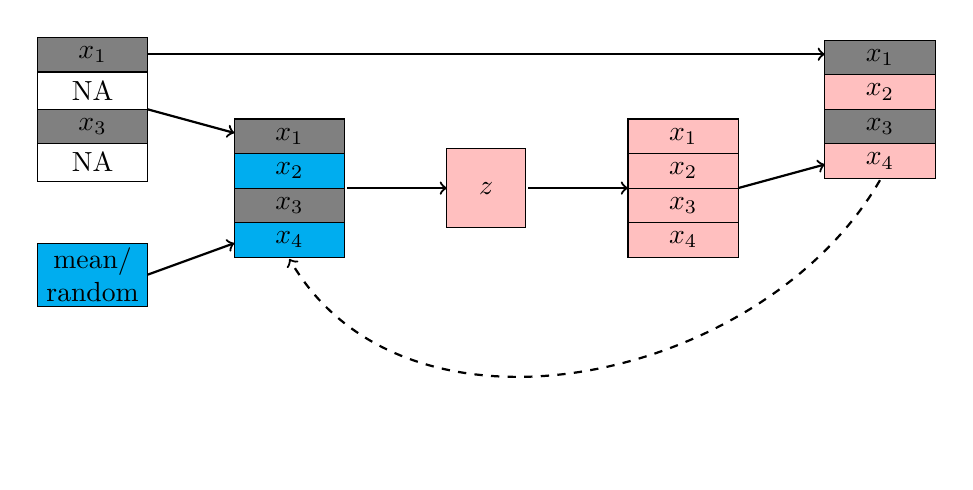
\begin{tikzpicture}
\measbox (0,0.5) rectangle (12,6.5);
\def\xx#1#2#3{
    \matrix [at={#1},style={nodes={rectangle,draw,minimum width=1.4cm,minimum height=1.2em}}, row sep=-\pgflinewidth]
        {
            \node[fill=#2] {$x_1$}; \\
            \node[fill=#3] {\xa}; \\
            \node[fill=#2] {$x_3$}; \\
            \node[fill=#3] {\xb}; \\
        };
}

    \def\xa{NA} \def\xb{NA}
    \draw[fill=cyan] (0.3,2.0) rectangle (1.7,2.8);
    \node[align=center] at (1.0,2.4) {mean/ \\ random};
    \xx{(1,4.5)}{gray}{white}
    \def\xa{$x_2$} \def\xb{$x_4$}
    \xx{(3.5,3.5)}{gray}{cyan}
    \draw[fill=pink] (5.5,3.0) rectangle (6.5,4.0);
    \node at (6.0,3.5) {$z$};
    %\node[at={(5.5,4)},draw,rectangle,width=5] {z};
    \xx{(8.5,3.5)}{pink}{pink}
    \xx{(11,4.5)}{gray}{pink}
    \draw[->,thick] (1.7,5.2) -- (10.3,5.2);
    \draw[->,thick] (1.7,4.5) -- (2.8,4.2);
    \draw[->,thick] (1.7,2.4) -- (2.8,2.8);
    \draw[->,thick] (4.23,3.5) -- (5.5,3.5);
    \draw[->,thick] (6.53,3.5) -- (7.8,3.5);
    \draw[->,thick] (9.20,3.5) -- (10.3,3.8);
    \draw[->,thick,dashed] (11.0,3.6) to[in=-60,out=-120] (3.5,2.6);

\end{tikzpicture}
\end{document}
